\section{Exercise 1} \label{P1}
% Write some intro

From the previous assignment are implemented the same functions \verb*|geometricModel| and \verb*|kinematicModel| with some differences.
In the \verb*|geometricModel| is added a function \verb*|getToolTransformWrtBase| that compute the tool transformation matrix with respect to the base frame $^b_t T = ^b_e T \cdot ^e_t T$. The transformation matrix $^b_e T$ is computed as in the previous assignment with \verb*|getTransformWrtBase|.

\section{Exercise 2}
The Jacobian matrix in \verb*|kinematicModel| due to the presents of the tool is 
\begin{equation} \label{E1}
	^b_t J = ^b \mathbb{S}_{t/e} \cdot ^b J_{e/b}
\end{equation}
where $^b J_{e/b}$ is the basic Jacobian matrix and $^b \mathbb{S}_{t/e} \in \mathbb{R}^{6\times6}$ is the rigid body Jacobian matrix 
\begin{equation*}
	^b \mathbb{S}_{t/e} = \begin{pmatrix}
		I_{3\times 3} & O_{3\times 3}  \\
		[^b \mathbf{r}_{t/e}\times]^\top & I_{3\times 3}
	\end{pmatrix}
\end{equation*}
where $^b \mathbf{r}_{t/e} = ^b \mathbf{r}_{t/b} - ^b \mathbf{r}_{e/b}$.

\subsection{Q2.1}
From $^b \boldsymbol\eta_{g}$ it is computed $^b_g R = ^b_g R_z(\boldsymbol\eta_{g,\mathbf k}) \cdot ^b_g R_y(\boldsymbol\eta_{g,\mathbf j}) \cdot ^b_g R_x(\boldsymbol\eta_{g,\mathbf i})$, checking if it is a proper rotation matrix. Then it is possible to obtain the transformation matrix
\begin{equation*} \renewcommand{\arraystretch}{1.5}
	^b_g T = \begin{pmatrix}
		^b_g R & ^b \mathbf{O}_{g} \\
		\mathbf{O}_{1 \times 3} & 1
	\end{pmatrix}
\end{equation*}
It is implemented the new class \verb*|cartesianControl|, where is present a function \verb*|getCartesianReference| that given the $^b_g T$ computes the Cartesian error.
This function at first compute $^t_g T = {} ^b_t T^{-1} \cdot ^b_g T$, and then obtain $^t\mathbf{h}_{g/t}$ and $\theta$ from $^t_g R$.
The Cartesian error between the robot end-effector frame and the goal frame is
\begin{equation*} \renewcommand{\arraystretch}{1.5}
	^b \mathbf{e}_{t/g} = \begin{pmatrix}
		^b \boldsymbol\rho_{t/g} \\ 
		^b \mathbf{r}_{t/g}
	\end{pmatrix} = \begin{pmatrix}
		^b_t R \cdot ^t\mathbf{h}_{g/t} \cdot \theta \\ 
		^b \mathbf{r}_{g/b} - ^b \mathbf{r}_{t/b}
	\end{pmatrix}
\end{equation*}
where $^b_t R$ is obtained by $^b_t T$ from the Section \ref{P1} with the function \verb*|getTransformWrtBase|.

\subsection{Q2.2}
Desired angular and linear reference velocities of the end-effector  with respect to the base are computed as follow
\begin{equation*}
	^b \boldsymbol\nu^*_{t/0} = \begin{bmatrix}
		\kappa_a &0\\
		0 &\kappa_l
	\end{bmatrix}\cdot 	^b \mathbf{e}_{t/g}
\end{equation*}
where $\kappa_{a} = 0.8$, $\kappa_{l} = 0.8$ are the gain.

\subsection{Q2.3}
The desired joint velocities are computed with the following equation
\begin{equation*}
	\dot{\bar{\mathbf{q}}} = ^b_t J ^\dagger \cdot ^b \boldsymbol\nu^*_{t/0}
\end{equation*}
where $^b_t J ^\dagger$ is the pseudoinverse of the Jacobian matrix computed with the Equation \ref{E1}.

\subsection{Q2.4}
The simulation of the robot's motion is implemented in the function \verb*|KinematicSimulation|. It takes in input: 
\begin{itemize}
	\item the current robot configuration (vector of joint positions) $\mathbf{q}$;
	\item the joints velocity $\dot{\bar{\mathbf{q}}}$;
	\item sample time $t_{s} = \frac{t_{\text{end}} - t_{\text{start}}}{\text{Number of samples}} = 0.1 \,s$;
	\item lower joint bounds $\mathbf{q_{\text{min}}}$;
	\item upper joint bounds $\mathbf{q_{\text{max}}}$.
\end{itemize}
And update $q_{i}$, where $i$ is the $i$-th joint, with the new value $q_{i} + \dot{\bar{q_{i}}} \cdot t_{s}$, if it is not greater of $\mathbf{q_{\text{max}}}$ and lower than $\mathbf{q_{\text{min}}}$. \\
During the simulation the robot's tool moves directly to the goal, see Figure \ref{fig:finalconfiguration} and \ref{fig:motionofthemanipulator}. This is coherent with the graph in Figure \ref{fig:directionvelocitiesee}, indeed both angular and linear velocities are constant, this means that the tool configuration changes constantly (without variation of the velocities).

\begin{figure}
	\centering
	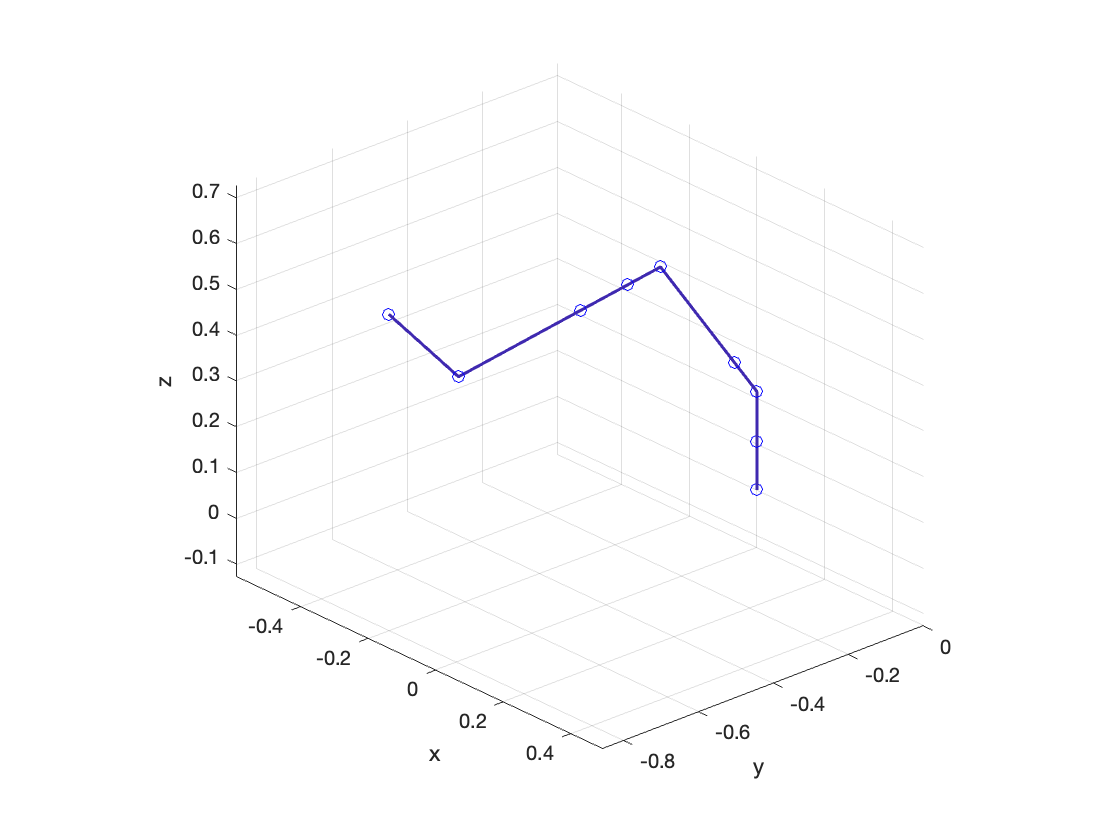
\includegraphics[width=0.7\linewidth]{Resources/FinalConfiguration}
	\caption{Final configuration of the robot during simulated motion in a three-dimensional graph. The measurement units for the three axes are meters.}
	\label{fig:finalconfiguration}
\end{figure}
\begin{figure}
	\centering
	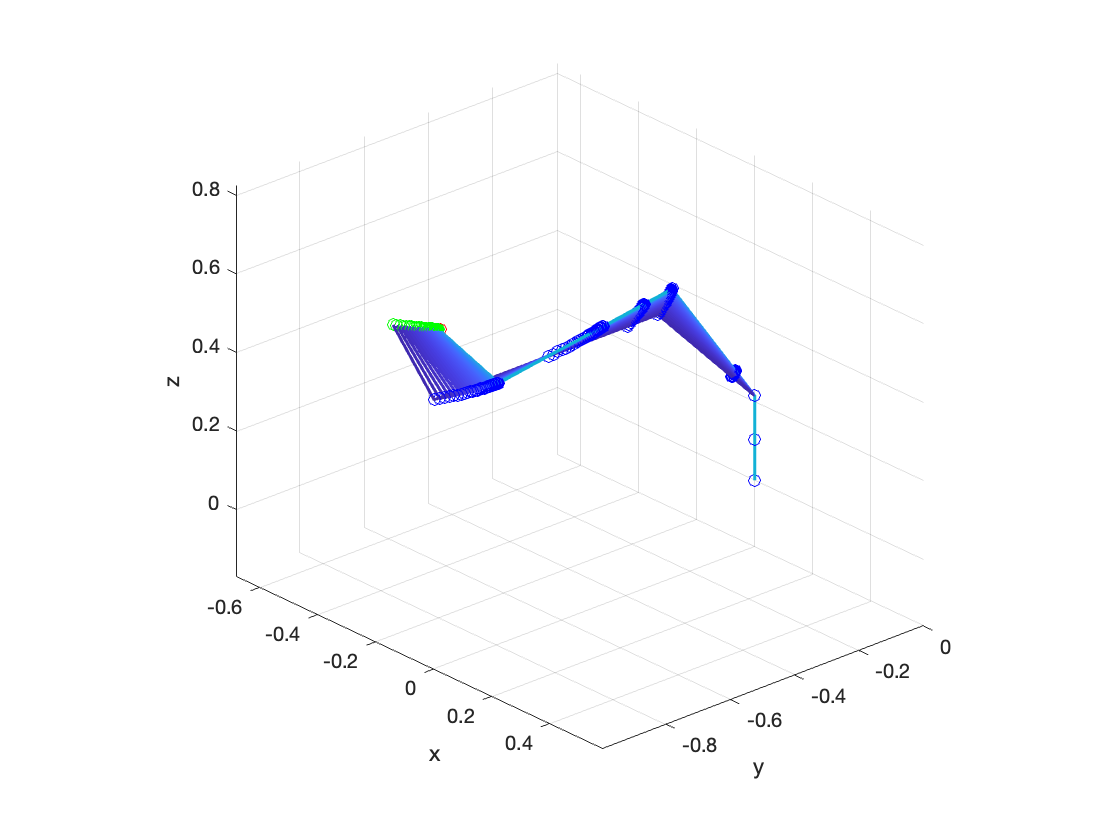
\includegraphics[width=0.7\linewidth]{Resources/MotionOfTheManipulator}
	\caption{ Description of the manipulator’s simulation motion in a three-dimensional graph. The horizontal axes, denoted by x and y, represent the horizontal motion, while the vertical axis, denoted by z, represents the vertical motion. The measurement units for all three axes are meters.}
	\label{fig:motionofthemanipulator}
\end{figure}
\begin{figure}
	\centering
	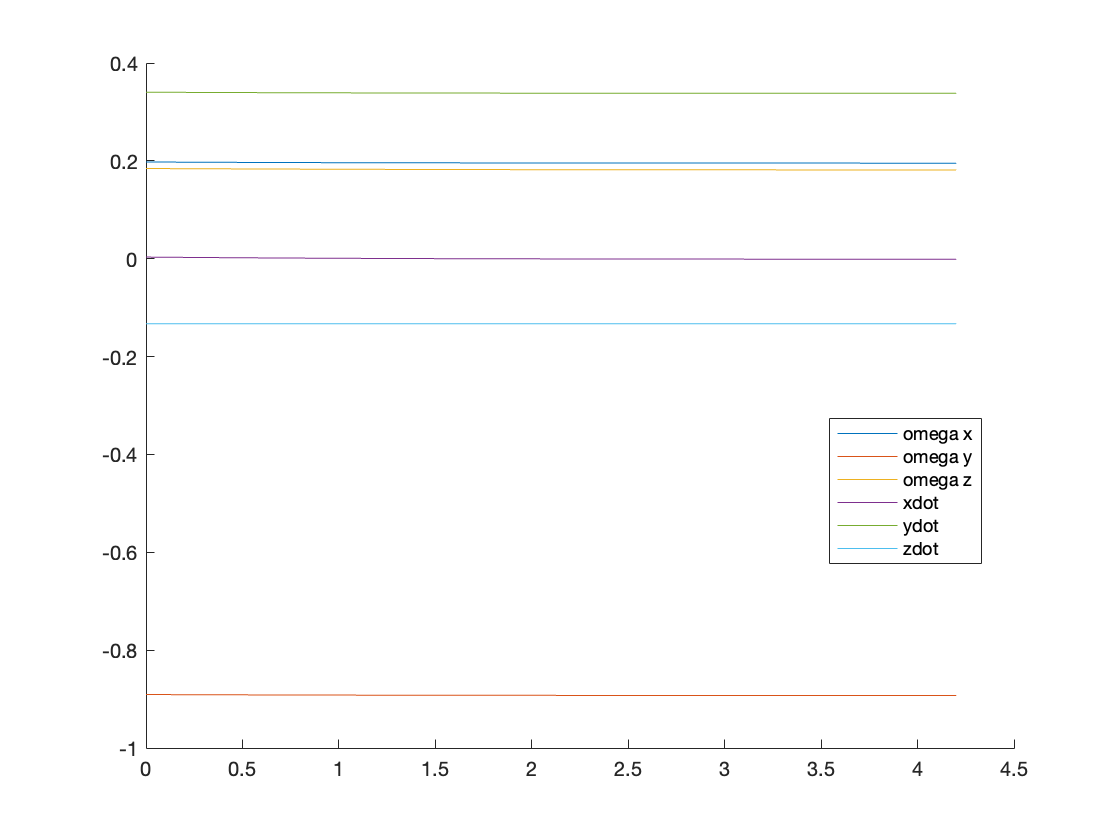
\includegraphics[width=0.7\linewidth]{Resources/DirectionVelocitiesEE}
	\caption{Envelope of end-effector angular ($\frac{rad}{s}$) and linear ($\frac{m}{s}$) velocities' direction.}
	\label{fig:directionvelocitiesee}
\end{figure}
